\sloppy
\chapter{Элементы теории графов}
\section{О том, как появилась теория графов...}

\mysubsection{История развития}
	Путь, по которому развивается любая область математики можно сравнить с русскими дорогами: то там, то здесь встретится выбоина, в которую если попадешь, то выбраться сможешь не скоро. Под этими <<выбоинами>> можно понимать великие математические загадки: формулировки у них простые, а вот доказательства~---~нет.
	
	Неоднократны случаи, когда математические задачи искали своего решения не одно столетие, а некоторые из них до сих пор его и не нашли. Стоит только вспомнить нашумевшую в конце XX века Великую теорему Ферма, которую всё-таки смог в $1994$ году доказать Эндрю Уайлс. Однако, как показала практика, между доказанной и недоказанной теоремой мало отличий, с практической точки зрения, а значит, и пользы должны быть мало от этого. Так, почему же за их решение часто дают престижные премии и так почитают математиков, которые смогли одолеть эти задачи?
	
	Дело в том, что какая-то задача становится великой в тот момент, когда существующего математического аппарата не хватает для её решения. В этом ключе великие задачи похожи на высокие крепостные стены, которые видны из далека и до которых путь не близок. И преодолевая этот путь, исследователи совершенствуют свой рабочий инструмент, открывая удивительные возможности математики. Именно по такому пути и начала своё развитие теория графов.

	Достоверно известно, что впервые эта теория была затронута в одной из работ Леонарда Эйлера, опубликованной в $1736$ году. В ней Эйлер сформулировал и решил <<Задачу о семи кёнигсбергских мостах>>. Как и всегда, математические головоломки использовались скорее в качестве развлечения и не предвещали новые открытия, поэтому долгое время теория графов не имела широкого применения и не воспринималась всерьёз.  

	Однако некоторые всё-таки преуспели в этом деле. Так, например, в $1852$ году Фрэнсисом Гутри была сформулирована гипотеза о четырёх красках. Понадобилось почти $120$ лет, чтобы решить её. Позже мы ещё вернемся к ней и обсудим преграды, которые возникли на пути математиков в процессе решения этой задачи.
	
	В XIX веке произошёл значительный скачок в теории графов, связанный с развитием теории электрических цепей и органической химии. В~$1847$ году Густав Кирхгов доказал матричную теорему о деревьях, а в~$1889$ году Артур Кэли, английский математик, доказал одноименную теорему о числе остовных деревьев полного графа. С начала $30$-х годов XIX века математики, как голодные звери, постепенно стягивались на эту сладкую и новую область, в которой, как оказалось, далеко не всё было очевидным.
	
	Несмотря на бурное развитие этой теории, до XX века она представляла из себя очень разрозненные области, которые имели общим началом только сам граф. С середины XX века появились успешные попытки структуризовать её: в частности, в этом деле преуспели К. Берж, О. Оре, Ф. Харари. Ещё один рывок в этом направлении был сделан совсем недавно, около 30 лет назад, Тимом Бернерс-Ли, который создал Интернет. Впоследствии, как мы знаем, Всемирная паутина обрела невероятные масштабы и теперь все передачи, шифрование основано на алгоритмах на графах.
	
	Благодаря элегантному, стройному виду, в который облачили теорию графов математики середины и конца XX века, её начали активно использовать при составлении олимпиад для школьников и студентов, включили во многие студенческие программы. Такая практика только укрепила фундамент этой теории и дала толчок к появлению большого числа методических пособий, направленных на неподготовленного читателя. До сих пор скорость развития теории графов не снизилась и всё большее число математиков устремляют свой взгляд в сторону графов.
\begin{paracol}{2}
	Как мы только что поняли, в становлении теории графов большую роль сыграла практика. Как именно? Когда специалист сталкивался с какими-то операциями, связями, отношениями, он пытался их изобразить в качестве рисунка. При этом суть самих вещей опускалась, то есть было не важно, как изобразить объект, поэтому было удобно для этого на рисунке поставить просто точку.
	
	Далее надо было указать отношения между этими точками и вполне логично было соединять точки линиями. В некоторых ситуациях, чтобы указать отличительную особенность отношений между объектами, стоило рисовать вместо линии стрелку.
	
	Таким образом, и начали появлятся графы~---~рисунки с вершинами, некоторые из которых соединены линиями.
	 
\switchcolumn

\begin{tikzpicture}
	\path (144:1.5) edge [bend right=45](216:1.5)
    	  (144:1.5) edge [bend left=30] (288:1.5);	
   	 
	\Loop [dist=2cm, dir=EA](0:1.5);
	\Loop [dist=2cm, dir=NO](72:1.5);
	\Loop [dist=2cm, dir=NOWE](144:1.5);
	\Loop [dist=2cm, dir=SOWE](216:1.5);
	\Loop [dist=2cm, dir=SOEA](288:1.5);
	
	\Loop [dist=2cm, dir=NO](260:5);  
	
	\tikzstyle{every node}=[circle, draw, fill=red, inner sep=0pt, minimum width=6pt]
	
	\foreach \x in {0,72,...,288}
    {
    	\draw [->, >=stealth']
    	(\x:1.5) node {} -- (\x+72:1.5)
    	(\x:1.5) node {} -- (\x+144:1.5)
    	(\x:1.5) node {} -- (\x+216:1.5)
    	(\x:1.5) node {} -- (\x+288:1.5);
    };
    
    \draw (255:2.5) node {} -- (285:4.5) node {} -- (265:6) node {} -- (260:5) node {};
      
    
    \draw \foreach \x in {0,72,...,288}
    {
    	(\x:1.5) node {}
    };
\end{tikzpicture}\begin{center}
	Рис. 1. Абсолютно произвольный граф 
\end{center}\end{paracol}
	
	После того, как задача формулировалась на языке теории графов, математики указывали параметры, которые были весомыми в рамках поставленной задачи. Так, в каких-то задачах надо было изображать ориентированные графы, в других~---~планарные, в тех, которые были связаны с сетями,~---~взвешенные, случайные. С помощью расширения области применения графов вариативность графов расширялась, открывая невероятные миры перед математиком.	 

	Математики отвечали взаимностью на такое разнообразие графов: у них появлялось невероятное число вопросов, на которые должна была ответить теория графов. Смешение возможностей этой новой области и рвения самых любопытных математиков привело к тому, что графы заняли одно из самых главных мест в комбинаторике. 
	
	Мать теории графов~---~комбинаторика~---~начала своё существование более двух тысячелетий назад, хотя сам термин был введён только в $1666$ году Лейбницем. Этот раздел математики сильно расширил свои владения, завладев частью теорий экстремальных задач, топологии, теории вероятностей. Кроме такой экспансии, она породила ещё несколько своих направлений: теорию графов, теорию Рамсея, перечислительную комбинаторику. Последуем же в след названию этой книги и окунёмся в мир теоретико-графовых моделей!
	
\mysubsection{Примеры}	
	
	Разберём два примера, которые можно отнести к самому нижнему ярусу школьной олимпиадной математики. Они покажут нам, как с помощью несложных рассуждений в рамках теории графов можно буквально разломить задачу и достать искомый ответ.
	
	Оба примера позаимствованы из книги <<Ленинградские математические кружки>>, в которой любознательный читатель может найти много схожих интересных задач. В этой книге также увлекательно изложены многие темы, которые было бы полезно освоить начинающему олимпиаднику.
\begin{example}
	Между $9$-ю городами России введены участки высокоскоростной автомагистрали. Есть следующие марщруты: Москва~---~Казань, Владивосток~---~Архангельск, Москва~---~Владивосток, Владивосток~---~Казань, Казань~---~Архангельск, Грозный~---~Смоленск, Смоленск~---~Новгород, Новгород~---~Углич, Углич~---~Тверь и Тверь~---~Грозный. Можно ли добраться из Москвы до Твери?

	\emph{Решение.} Нарисуем схему: городами будут соответственно точки, а соединяющим их дорогами~---~непересекающиеся между собой линии (см. рис. $2$). Теперь видно, что доехать от Москвы до Твери нельзя.

\begin{center}\begin{tikzpicture}
		[shorten >=1pt,auto,node distance=1.7cm, thick, main node/.style={circle,draw, font=\sffamily}]
  		
		\node[main node] (Z) 		   	   {М};
  		\node[main node] (P)  [below of=Z] {В};
  		\node[main node] (Me) [right of=Z] {К};
  		\node[main node] (V)  [right of=P] {А};
  		
 		\draw
    	(Z)  -- (Me)
    	(Me) -- (P)
    	(P)  -- (Z)
    	(P)  -- (V)
    	(V)  -- (Me);
    	
    	\draw (4, -2.5) node {Рис. 2.};
    	\draw (4, -3) node {\small Высокоскоростные магистрали};
\end{tikzpicture}
\begin{tikzpicture}
		[shorten >=1pt,auto,node distance=1.7cm, thick, main node/.style={circle,draw, font=\sffamily}]
  		
  		\node[main node] (U)  [] {Г};
  		\node[main node] (N)  [above of=U] {С};
  		\node[main node] (S)  [right of=N] {Н};
  		\node[main node] (Ma) [right of=U] {Т};
  		\node[main node] (J)  [below right of=S] {У};
  		
 		\draw
    	(U)  -- (N)
    	(N)  -- (S)
    	(S)  -- (J)
    	(J)  -- (Ma)
    	(Ma) -- (U);
    	
    	\draw (0, -1.5) node {};
\end{tikzpicture}\end{center}
\end{example}

\begin{example}
Можно ли за несколько ходов из исходного положения (см. рис. $3$) получить такую же картину, как на рис. $4$? 

\begin{paracol}{2}
	Занумеруем поля шахматной доски так, как показано на рис. $5$. И представим её в виде графа, в котором будет $9$ вершин и соединены будут те из них, которые могут быть последовательными клетками пути коня, то есть отстающие друг от друга на две клетки по вертикали и одну по горизонтали или наоборот. 
	
	Начальная и конечная расстановки изображены соответственно на рис. $6$ и на рис.~$7$. Очевидно, что порядок следования коней измениться не может, поэтому переставить коней не получится.
\switchcolumn
\begin{center}
\begin{tikzpicture}
	\draw[dashed] (0,0)rectangle (0.5,-0.5);
	\draw[dashed] (0.5,0)rectangle (1,-0.5);
	\draw[dashed] (1,0)rectangle (1.5,-0.5);

	\draw[dashed] (0,-0.5)rectangle (0.5,-1);
	\draw[dashed] (0.5,-0.5)rectangle (1,-1);
	\draw[dashed] (1,-0.5)rectangle (1.5,-1);
	
	\draw[dashed] (0,-1)rectangle (0.5,-1.5);
	\draw[dashed] (0.5,-1)rectangle (1,-1.5);
	\draw[dashed] (1,-1)rectangle (1.5,-1.5);

	\node at (0.25, -0.25)[] {
\includegraphics[width=1in,%
height=0.4cm,keepaspectratio]{sections/images/white_hourse}};
	\node at (1.25, -0.25)[] {
\includegraphics[width=1in,%
height=0.4cm,keepaspectratio]{sections/images/white_hourse}};
	\node at (1.25, -1.25)[] {
\includegraphics[width=1in,%
height=0.4cm,keepaspectratio]{sections/images/black_hourse}};
	\node at (0.25, -1.25)[] {
\includegraphics[width=1in,%
height=0.4cm,keepaspectratio]{sections/images/black_hourse}};		
	\draw (0.75, -2) node []  {\small Рис. 3};
\end{tikzpicture}
\;\ \;\ \;\
\begin{tikzpicture}    
	\draw[dashed] (0,0)rectangle (0.5,-0.5);
	\draw[dashed] (0.5,0)rectangle (1,-0.5);
	\draw[dashed] (1,0)rectangle (1.5,-0.5);

	\draw[dashed] (0,-0.5)rectangle (0.5,-1);
	\draw[dashed] (0.5,-0.5)rectangle (1,-1);
	\draw[dashed] (1,-0.5)rectangle (1.5,-1);
	
	\draw[dashed] (0,-1)rectangle (0.5,-1.5);
	\draw[dashed] (0.5,-1)rectangle (1,-1.5);
	\draw[dashed] (1,-1)rectangle (1.5,-1.5);

	\node at (0.25, -0.25)[] {
\includegraphics[width=1in,%
height=0.4cm,keepaspectratio]{sections/images/white_hourse}};
	\node at (1.25, -0.25)[] {
\includegraphics[width=1in,%
height=0.4cm,keepaspectratio]{sections/images/black_hourse}};
	\node at (1.25, -1.25)[] {
\includegraphics[width=1in,%
height=0.4cm,keepaspectratio]{sections/images/white_hourse}};
	\node at (0.25, -1.25)[] {
\includegraphics[width=1in,%
height=0.4cm,keepaspectratio]{sections/images/black_hourse}};		
	\draw (0.75, -2) node []  {\small Рис. 4};
\end{tikzpicture}

\begin{tikzpicture}    
	\draw[dashed] (0,0)rectangle (0.5,-0.5);
	\draw[dashed] (0.5,0)rectangle (1,-0.5);
	\draw[dashed] (1,0)rectangle (1.5,-0.5);

	\draw[dashed] (0,-0.5)rectangle (0.5,-1);
	\draw[dashed] (0.5,-0.5)rectangle (1,-1);
	\draw[dashed] (1,-0.5)rectangle (1.5,-1);
	
	\draw[dashed] (0,-1)rectangle (0.5,-1.5);
	\draw[dashed] (0.5,-1)rectangle (1,-1.5);
	\draw[dashed] (1,-1)rectangle (1.5,-1.5);

	\node at (0.25, -0.25)[] {1};
	\node at (0.25, -0.75)[] {2};
	\node at (0.25, -1.25)[] {3};
	
	\node at (0.75, -0.25)[] {4};
	\node at (0.75, -0.75)[] {5};
	\node at (0.75, -1.25)[] {6};
	
	\node at (1.25, -0.25)[] {7};
	\node at (1.25, -0.75)[] {8};
	\node at (1.25, -1.25)[] {9};
	
	\draw (0.75, -2) node []  {\small Рис. 5};
\end{tikzpicture}\end{center}
\end{paracol}
\begin{center}\begin{tikzpicture}
		[shorten >=1pt,auto,node distance=1.3cm, thick, main node/.style={circle,draw, font=\sffamily}]
  		
  		\node[main node] (a)  [] {
\includegraphics[width=1in,%
height=0.4cm,keepaspectratio]{sections/images/white_hourse}};
  		\node[main node] (b)  [above of=a] {6};
  		\node[main node] (c)  [above right of=b] {
\includegraphics[width=1in,%
height=0.4cm,keepaspectratio]{sections/images/white_hourse}};
  		\node[main node] (d) [right of=c] {2};
  		\node[main node] (e)  [right of=d] {
\includegraphics[width=1in,%
height=0.4cm,keepaspectratio]{sections/images/black_hourse}};
  		\node[main node] (f)  [below of=e] {4};
  		\node[main node] (g)  [below left of=f] {
\includegraphics[width=1in,%
height=0.4cm,keepaspectratio]{sections/images/black_hourse}};
  		\node[main node] (h)  [left of=g] {8};
  		
  		\node[main node] (i)  [right of=g] {5};
  		
 		\draw (a)  -- (b) -- (c) -- (d) -- (e) -- (f) -- (g) -- (h) -- (a);
\end{tikzpicture}
\;\ \;\ \;\ \;\ \;\ \;\ \;\ \;\ \;\ \;\
\begin{tikzpicture}
		[shorten >=1pt,auto,node distance=1.3cm, thick, main node/.style={circle,draw, font=\sffamily}]
  		
  		\node[main node] (a)  [] {
\includegraphics[width=1in,%
height=0.4cm,keepaspectratio]{sections/images/white_hourse}};
  		\node[main node] (b)  [above of=a] {6};
  		\node[main node] (c)  [above right of=b] {
\includegraphics[width=1in,%
height=0.4cm,keepaspectratio]{sections/images/black_hourse}};
  		\node[main node] (d) [right of=c] {2};
  		\node[main node] (e)  [right of=d] {
\includegraphics[width=1in,%
height=0.4cm,keepaspectratio]{sections/images/white_hourse}};
  		\node[main node] (f)  [below of=e] {4};
  		\node[main node] (g)  [below left of=f] {
\includegraphics[width=1in,%
height=0.4cm,keepaspectratio]{sections/images/black_hourse}};
  		\node[main node] (h)  [left of=g] {8};
  		
  		\node[main node] (i)  [right of=g] {5};
  		
 		\draw (a)  -- (b) -- (c) -- (d) -- (e) -- (f) -- (g) -- (h) -- (a);
\end{tikzpicture}\newline 
Рис. 6  \;\ \;\ \;\ \;\ \;\ \;\ \;\ \;\ \;\ \;\ \;\ \;\ \;\ \;\ \;\ \;\ \;\ \;\ \;\ \;\ \;\ \;\ \;\ \;\ \;\ Рис. $7$ \;\ \;\ \;\ \;\ \;\ \;\ 
\end{center}
\end{example}

\mysubsection{Великие математические задачи}

	Мы уже много слов сказали о том, как великие математические задачи привносят существенное влияние на развитие математики, в том числе и теории графов. Теперь остановимся на нескольких задачах, разберёмся в том, что они из себя представляют, и поговорим о том, как они подействовали на процесс становления теории графов.

	\textbf{Проблема семи мостов Кёнигсберга} была решена Эйлером в $1736$ году. Это считается отправной точкой появления теории графов. В этой задаче спрашивалось, можно ли пройти по всем семи мостам Кёнигсберга, не проходя ни по какому из них дважды. Многие жители любили эту загадку, но никто не мог ни решить её, ни опровергнуть. 
	
	Эйлер, в свою очередь, переформулировал эту задачу в терминах теории графов: можно ли выйти из какой-то вершины графа и пройти по всем ребрам графа ровно по одному разу. Граф, в котором так можно сделать, называется эйлеровым в честь своего первооткрывателя. 

	На самом деле, как, может, знает любознательный читатель, эйлеров граф~---~это граф, который можно нарисовать на бумаге, не отрывая карандаша. Таким образом, все рисунки из детских раскрасок, у которых надо было нарисовать контур, не отрывая карандаша от бумаги, есть ни что иное, как изображение эйлерового графа. 

\begin{center}
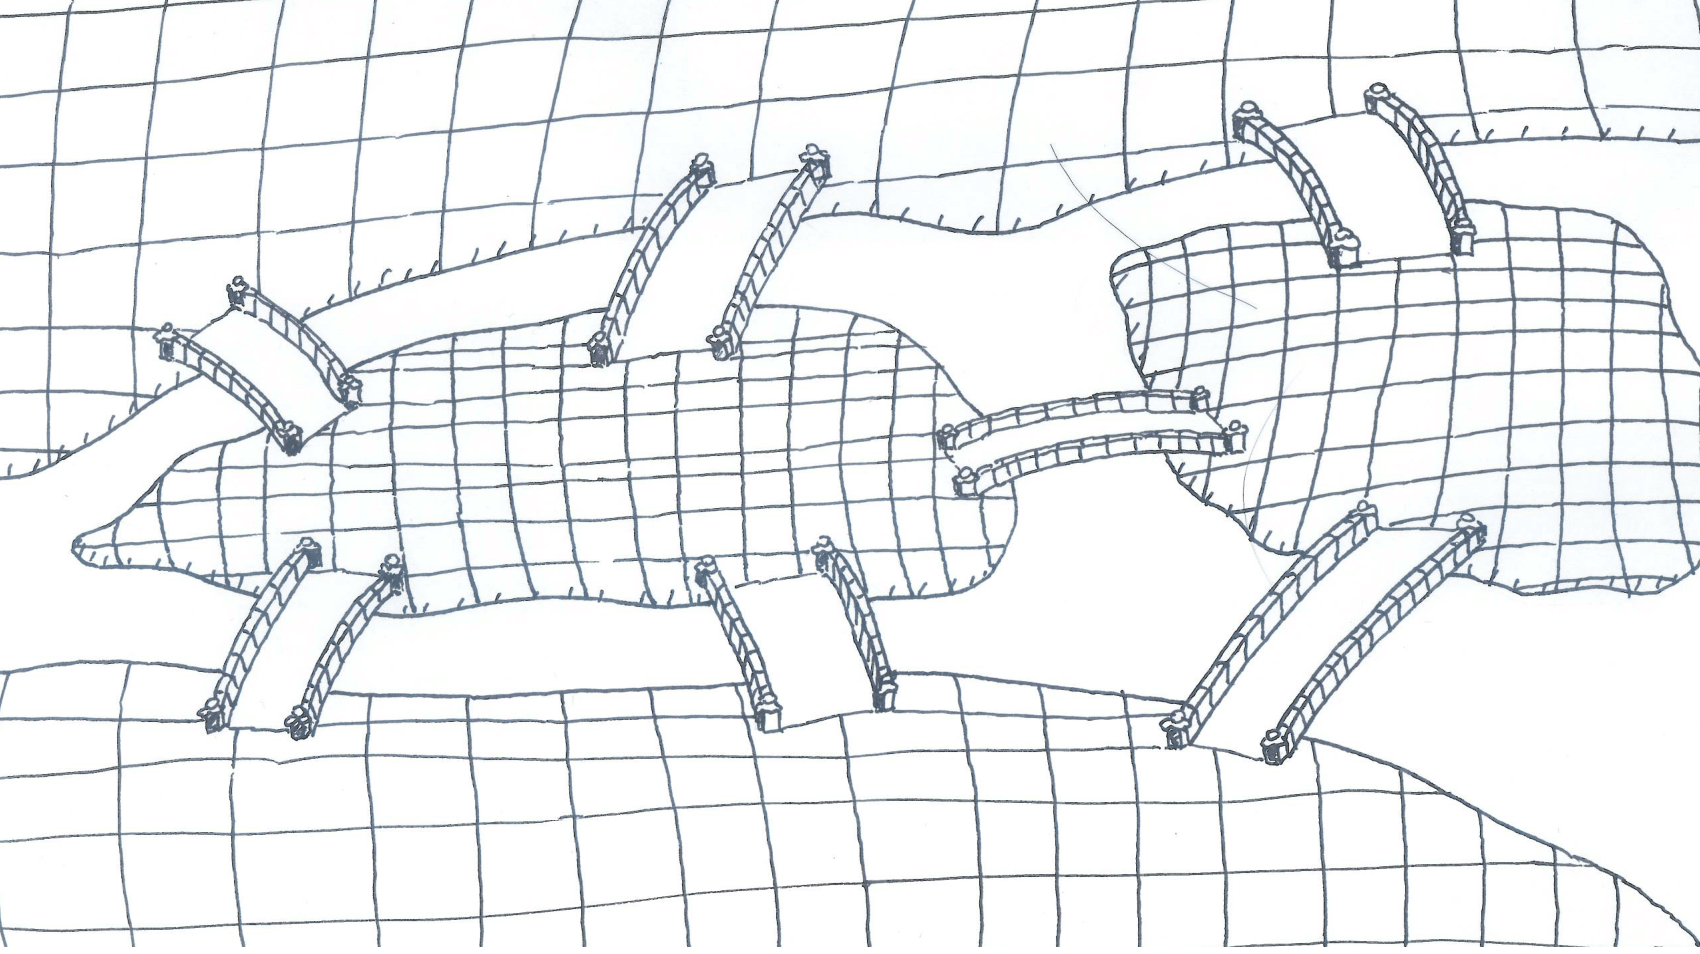
\includegraphics[width=8cm, height=9cm,keepaspectratio]{sections/images/Keningsberg}
\;\ \;\ \;\ \;\ \;\ \;\ \;\ \;\ \;\ \;\
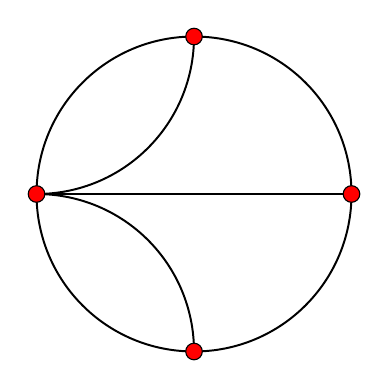
\begin{tikzpicture}
	\tikzstyle{every node}=[circle, draw, fill=red, inner sep=0pt, minimum width=6pt]
    	  
   	\path (0, 0) edge [bend right=45, line width=0.25mm](2, 2)
    	  (0, 0) edge [bend left=45, line width=0.25mm] (2, 2)
    	  (0, 0) edge [bend right=45, line width=0.25mm](2, -2)
    	  (0, 0) edge [bend left=45, line width=0.25mm] (2, -2);	
    	  
	\draw (0, 0) edge [line width=0.25mm] (4, 0)
		  (2, 2) edge [bend left=45, line width=0.25mm] (4, 0)
		  (2, -2) edge [bend right=45, line width=0.25mm] (4, 0);
	
    \draw (0, 0) node {} 
    	  (2, -2) node {} 
    	  (2, 2) node {} 
    	  (4, 0) node {};

\end{tikzpicture}\end{center}

\begin{center}\small Рис. $8$. Кёнигсберг: схематически (слева) и графически (справа)\end{center}

	Эйлер в своей работе не только решил эту задачу, но и сформулировал критерий эйлеровости графа, что позволяет ответить на вопрос для любого графа: можно ли пройти по всем его рёбрам ровно один раз или нет. 
	
	Попробуте обойти следующий граф, а потом посчитайте количество рёбер, которое выходит из каждой вершины. Какое оно?
	
\begin{center}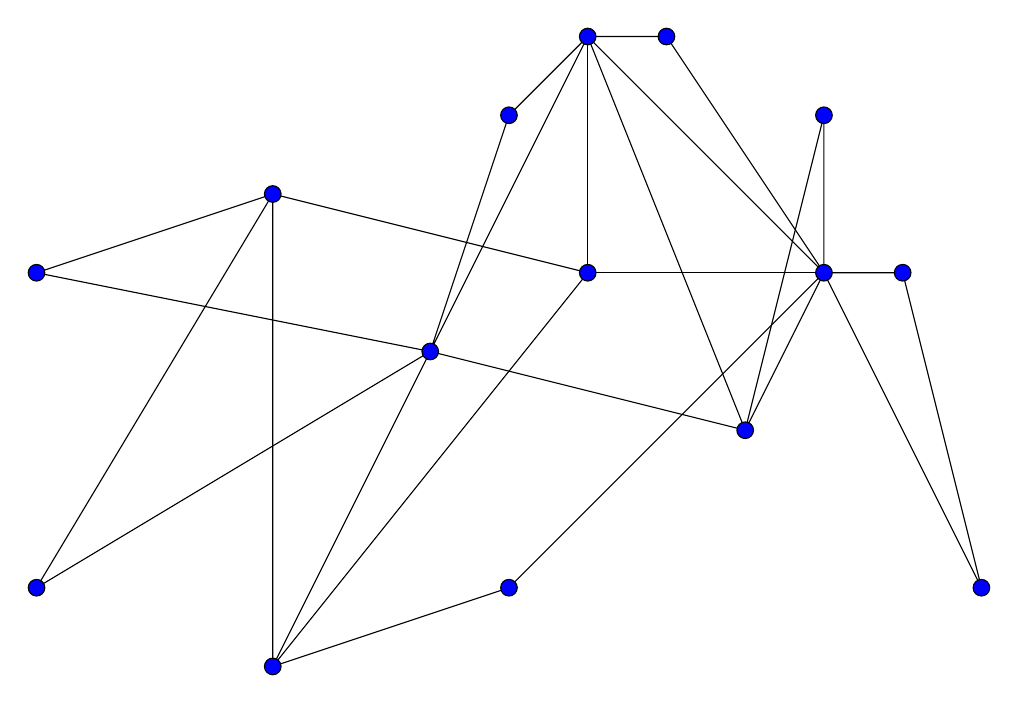
\begin{tikzpicture}
	\tikzstyle{every node}=[circle, draw, fill=blue, inner sep=0pt, minimum width=6pt]
    	  
	\draw (1, 2) -- (4, 7)
		  (1, 2) -- (6, 5);
		  
	\draw (1, 6) -- (4, 7)
		  (1, 6) -- (6, 5);

	\draw (4, 7) -- (4, 1)
		  (4, 7) -- (8, 6);

	\draw (4, 1) -- (6, 5)
		  (4, 1) --(8, 6)
		  (4, 1) -- (7, 2);
		  
	\draw (6, 5) -- (7, 8)
		  (6, 5) -- (8, 9)
		  (6, 5) -- (10, 4);
		  
	\draw (7, 2) -- (11, 6);
	
	\draw (7, 8) -- (8, 9);

	\draw (8, 6) -- (11, 6)
		  (8, 6) -- (8, 9);
		  
	\draw (8, 9) -- (9, 9)
		  (8, 9) -- (11, 6)
		  (8, 9) -- (10, 4);
		  
	\draw (9, 9) -- (11, 6);
	
	\draw (10, 4) -- (11, 6)
		  (10, 4) -- (11, 8);
		  
	\draw (11, 6) -- (11, 8)
		  (11, 6) -- (12, 6)
		  (11, 6) -- (13, 2);
		  
	\draw (12, 6) -- (13, 2);
	
    \draw (1, 2) node {} 
    	  (1, 6) node {} 
    	  (4, 7) node {} 
    	  (4, 1) node {} 
    	  (6, 5) node {} 
    	  (7, 2) node {} 
    	  (7, 8) node {} 
    	  (8, 6) node {} 
    	  (8, 9) node {} 
    	  (9, 9) node {} 
    	  (10, 4) node {} 
    	  (11, 6) node {} 
    	  (11, 8) node {} 
    	  (12, 6) node {} 
    	  (13, 2) node {};

\end{tikzpicture}\end{center}

\begin{center}\small Рис. $9$. Эйлеров граф\end{center}	
	
	Эйлеровы графы имеют в качестве <<собратьев по несчастью>> гамильтоновы графы~---~графы, в которых можно обойти все вершины, побывав в каждой ровно один раз. Однако несмотря на простоту первых из них, вторые не поддаются никакой классификации и до сих пор неизвестно, есть ли оптимальный алгоритм, который мог бы ответить на вопрос: гамильтонов ли наш граф или нет? Говоря об оптимальности, математики подразумевают достаточно формальные понятия. О них мы тоже упомянем немного ниже.
	
	Своим появлением гамильтонов цикл обязан задаче о коммивояжёре, в которой торговец должен был обойти все города, побывав в каждом ровно один раз. С тех пор появилось много задач, для решения которых нужно найти гамильтонов цикл, так что можно считать, что этот путь развития теории графов был вполне успешным.	
	
	Сам Гамильтон сформулировал и решил следующую задачу: можно ли обойти додекаэдр, побывав в каждой вершине единожды. Одно из решений есть на рис. 10.
	
\begin{center}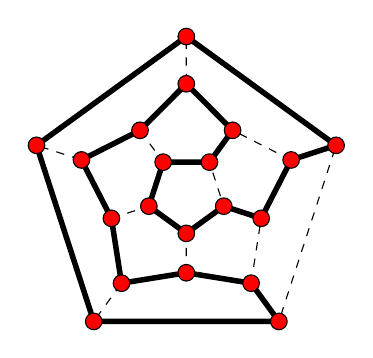
\begin{tikzpicture}
	\tikzstyle{every node}=[circle, draw, fill=red, inner sep=0pt, minimum width=6pt]	
	
	\draw [line width=0.7mm] (126:0.5) -- (198:0.5) -- (270:0.5) -- (342:0.5) -- (342:1.0) -- (18:1.4) -- (18:2.0) -- (90:2.0) -- (162:2.0) -- (234:2.0) -- (306:2.0) -- (306:1.4) -- (270:1.0) -- (234:1.4) -- (198:1.0) -- (162:1.4) -- (126:1.0) -- (90:1.4) -- (54:1.0) -- (54:0.5) -- (126:0.5);

    \draw [dashed]  \foreach \x in {54,126,...,342}
    {
    	
    	(\x:1.0) -- (\x:0.5) -- (\x+72:0.5)
    	(\x-36:1.4) -- (\x:1.0) -- (\x+36:1.4) -- (\x+36:2.0) -- (\x-36:2.0)
    };	
    \draw \foreach \x in {54,126,...,342}
    {
    	(\x:0.5) node {}
    	(\x:1.0) node {}
    };
    \draw \foreach \x in {18,90,...,306}
    {
    	(\x:1.4) node {}
    };
    \draw \foreach \x in {18,90,...,306}
    {
    	(\x:2.0) node {}
    };
\end{tikzpicture}

	\small Рис. 10. Гамильтонов цикл в додекаэдре
\end{center}
	
\begin{paracol}{2}
	\textbf{Теорема о четырёх красках} утверждает, что любую карту можно раскрасить в четыре цвета так, что любая страна раскрашена в один цвет, а соседние страны всегда раскрашены в разные цвета. Фрэнсис Гутри, сформулировавший эту задачу, изначально имел перед собой цель только раскрасить карту Англии. Он заметил, что меньше четырёх красок не хватит для этого. Можете ли вы посмотреть на схематический рисунок Великобритании и объяснить, почему меньше четырёх красок не хватит?
	
	В $1976$ году эту теорему успешно доказали Кеннет Аппел и Вольфганг Хакен, однако то решение, которое они предложили, вызвало сильный резонанс среди коллег. Дело было в том, что математики свели доказательство к проверке около двух тысяч графов на раскраску, но очень трудоёмко~---~проверять все эти случаи вручную, поэтому был написан машинный код, который и должен был справиться с задачей. Такой подход вызвал бурю возмущений среди их коллег...
\switchcolumn
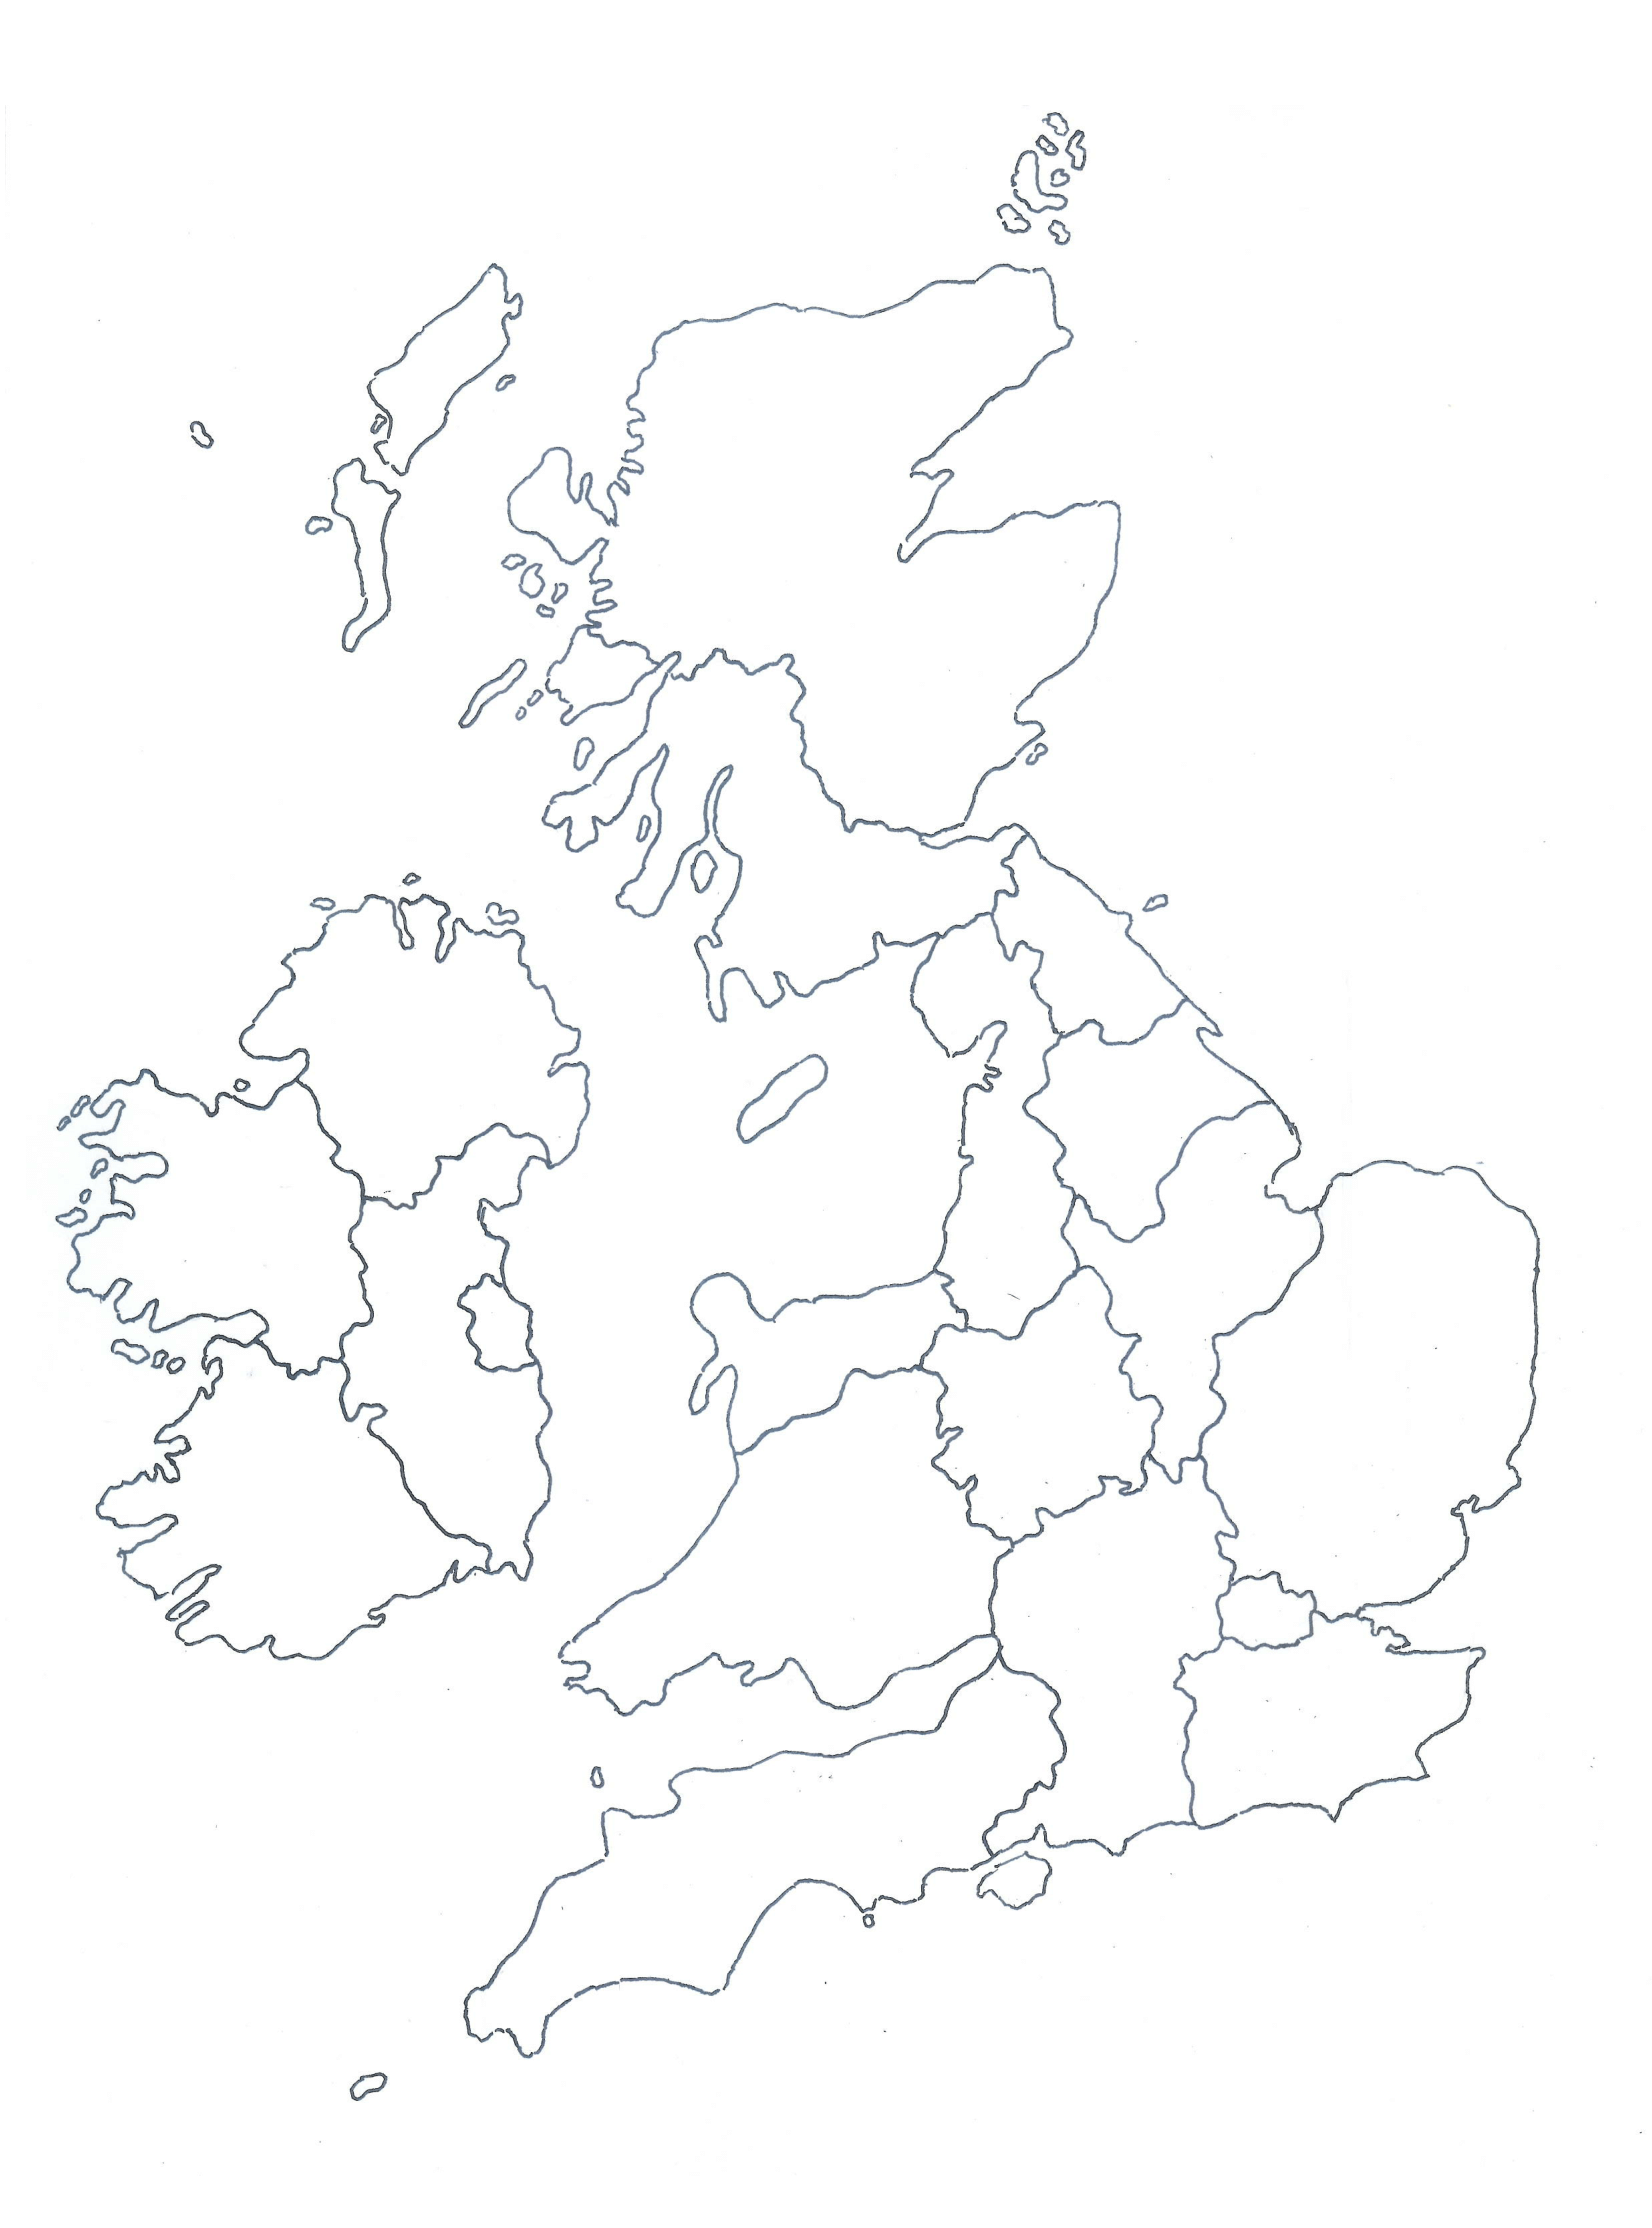
\includegraphics[width=8cm, height=24cm,keepaspectratio]{sections/images/England}
\begin{center}\small Рис. 11. Схематическое изображение частей Великобритании (пропорции не сохранены)\end{center}
\end{paracol}

	Фактически Аппел и Хакен поставили перед научным миром непростой вопрос: можно ли считать доказательство, использующее работу компьютера, строгим, правильным, с формальной точки зрения? 
	
	Долгое время всё сообщество не могло принять такой подход даже по отношению к теореме о четырёх красках, но в $1997$ году Робертсон, Сандерс, Сеймур и Томас предложили более простое доказательство теоремы, которое безвозвратно поместило эту теорему в список <<доказанных>>. К настоящему моменту почти все математики согласились с обоснованным использованием электронных носителей для завершения доказательства сложных теорем.
	
	\textbf{Задача о клике} была сформулирована в $1972$ году Ричардом Карпом. Причиной её появления можно считать дикое развитие теории вычислительных систем, начавшееся в середине $50$-х годов XX века и продолжающееся до сих пор. Условие у этой задачи следующее: предложите оптимальный алгоритм по нахождению максимального полного подграфа произвольного графа. Под полным подграфом подразумевается граф, в котором любые две вершины соединены ровно одни ребром и нет петель, то есть рёбер выходящих и входящих в одну и ту же вершину.
	
	По своей сути задача о клике говорит об оптимальном алгоритме. Ясно, что можно перебрать все возможные подграфы и проверить для каждого, является ли он полным, однако это не будет оптимальным алгоритмом. Критерий оптимальности в этом случае состоит в том, что время, которое мы тратим на работу алгоритма, есть функция, зависящая от длины входных данных. И по этому делению задача о клике относится к $NP$-полным задачам. В этот класс входят те задачи, которые за полиномиальное время не решаются, но любое их решение можно проверить на правильность за полиномиальное время.
	
\begin{center}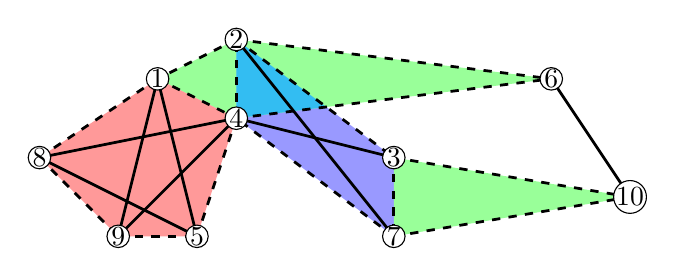
\begin{tikzpicture}
	\fill [draw=none, fill=green!40] (2, -0.5) -- (3, -1) -- (3, 0) -- (2, -0.5);
	\fill [draw=none, fill=blue!40] (5, -2.5) -- (3, -1) -- (3, 0) -- (5, -1.5);
	\fill [draw=none, fill=green!40] (3, -1) -- (3, 0) -- (7, -0.5);
	\fill [draw=none, fill=red!40] (2, -0.5) -- (3, -1) -- (2.5, -2.5) -- (1.5, -2.5)  -- (0.5, -1.5);
	\fill [draw=none, fill=green!40] (5, -1.5) -- (5, -2.5) -- (8, -2);
	
	\begin{scope}
		\clip (5, -2.5) -- (3, -1) -- (3, 0) -- (5, -1.5);
		\clip (3, -1) -- (3, 0) -- (7, -0.5);
		\fill[color=cyan!80] (3,0) rectangle (5,-2);
	\end{scope}	
	
	\draw (2, -0.5) edge [dashed, line width=0.35mm] (3, -1) 
		  (3, -1)   edge [dashed, line width=0.35mm] (3, 0) 
		  (3, 0)    edge [dashed, line width=0.35mm] (2, -0.5);

	\draw (3, -1)   edge [dashed, line width=0.35mm] (7, -0.5) 
		  (3, 0)    edge [dashed, line width=0.35mm] (7, -0.5);
	
	\draw (3, 0)    edge [dashed, line width=0.35mm] (5, -1.5) 
		  (5, -1.5) edge [dashed, line width=0.35mm] (5, -2.5) 
		  (5, -2.5) edge [dashed, line width=0.35mm] (3, -1)
		  (3, 0)  edge [line width=0.35mm] (5, -2.5) 
		  (3, -1) edge [line width=0.35mm] (5, -1.5);

	
	\draw (2, -0.5)   edge [dashed, line width=0.35mm] (0.5, -1.5) 
		  (0.5, -1.5) edge [dashed, line width=0.35mm] (1.5, -2.5) 
		  (1.5, -2.5) edge [dashed, line width=0.35mm] (2.5, -2.5)
		  (2.5, -2.5) edge [dashed, line width=0.35mm] (3, -1)
		  (2, -0.5)   edge [line width=0.35mm] (1.5, -2.5) 
		  (2, -0.5)   edge [line width=0.35mm] (2.5, -2.5)
		  (0.5, -1.5) edge [line width=0.35mm] (3, -1) 
		  (0.5, -1.5) edge [line width=0.35mm] (2.5, -2.5)
		  (1.5, -2.5) edge [line width=0.35mm] (3, -1);
		  
	\draw (5, -1.5) edge [dashed, line width=0.35mm] (8, -2) 
		  (5, -2.5) edge [dashed, line width=0.35mm] (8, -2);

	\draw (8, -2) edge [line width=0.35mm] (7, -0.5);
		  
	\draw (2, -0.5)   node[circle, draw, fill=white] {1}
		  (3, 0)      node[circle, draw, fill=white] {2}
		  (5, -1.5)   node[circle, draw, fill=white] {3}
		  (3, -1)     node[circle, draw, fill=white] {4}
		  (8, -2)     node[circle, draw, fill=white] {10}
		  (7, -0.5)   node[circle, draw, fill=white] {6}
		  (5, -2.5)   node[circle, draw, fill=white] {7}
		  (0.5, -1.5) node[circle, draw, fill=white] {8}
		  (1.5, -2.5) node[circle, draw, fill=white] {9}
		  (2.5, -2.5) node[circle, draw, fill=white] {5};
\end{tikzpicture}

	\small Рис. 12. Произвольный граф с изображенными кликами
\end{center}

	Это далеко не все задачи, которые встречались по ходу развития теории графов. К ним также можно отнести гипотезу Хадвигера, гипотезу Харари, гипотеза Конвея о трекле.
	
	Подытожим, в этом параграфе мы проследили за процессом становления теории графов, познакомились с неформальным определением графа и обсудили некоторые серьёзные теоремы, с которыми сталкивались математики по мере развития теории графов.